\section{Interrupts}
\subsection{Interrupt-Klassen}
\begin{itemize}
    \item Hardware-Fehler
    \item Timer
    \item I/O
    \item Software-Interrupts
    \begin{itemize}
        \item Arithmetik
        \item Traps
        \item etc.
    \end{itemize}
\end{itemize}

\subsection{Ablauf}
\begin{enumerate}
    \item Interrupt flag wird gesetzt
	\item Nach aktuellem Befehl wird unterbrochen (BS übernimmt Kontrolle)
	\item Prozess-Daten werden gespeichert (wie bei Kontextswitch)
	\item Mittels Interrupt-Vector wird die entsprechende ISR aufgerufen
	\item Diese ist nicht unterbrechbar und so kurz wie möglich
	\item Die ISR ruft dann ein sog. Tasklet auf welches unterbrechbar ist und die eigentliche Arbeit macht
\end{enumerate}

\subsection{Round Robin: I/O- vs CPU-lastig}
\textbf{CPU-lastinge} Prozesse nutzen ihre \textbf{Zeitquanten} vollständig, während \textbf{I/O}
Prozesse \textbf{warten} müssen.

\subsection{Interrupt Handling}
\begin{figure}[ht!]
    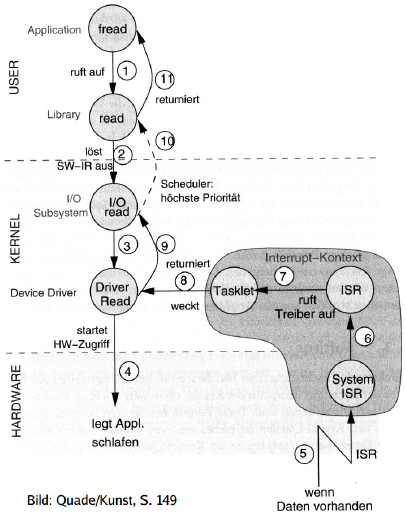
\includegraphics[scale=.8]{pics/isr}
    \caption{Interrupt callgraph}
\end{figure}